\section{问题四：非矩形模块布局模型的建立与求解}

本问沿着“外接矩形失效---真实形状集合---精确枚举---下界与构造共同证明最优”的主线，将问题一的矩形装箱模型推广到非矩形模块。

\subsection{几何模型：非矩形模块的形状级表示}

\subsubsection{模块形状解释}

问题四将问题一的矩形模块推广为 L 型、T 型等非矩形模块。矩形外接框不能反映凹槽的真实空闲区域，因此需要将每个模块表示为形状集合，并根据真实占用区域判断是否重叠。根据题面图 3 的标注与单位比例，采用表~\ref{tab:q4_shape_data} 所示的单位格解释。

\begin{table}[H]
  \centering
  \caption{图 3 四个模块的形状解释}
  \label{tab:q4_shape_data}
  \small
  \renewcommand{\arraystretch}{1.15}
  \begin{tabular}{c c c r p{6.0cm}}
    \toprule
    模块 & 类型 & 外接尺寸 & 面积 & 实际占用区域 \\
    \midrule
    b1 & T 型 & $4\times4$ & 12 & 上横为 $4\times2$，下竖为 $2\times2$ \\
    b2 & L 型 & $2\times4$ & 6 & 左竖为 $1\times4$，右下为 $1\times2$ \\
    b3 & 矩形 & $2\times1$ & 2 & 两个相邻单位格 \\
    b4 & 矩形 & $1\times4$ & 4 & 四个纵向相邻单位格 \\
    \bottomrule
  \end{tabular}
\end{table}

其中，题面未以独立文字表格给出 b1 的全部竖向尺寸。根据图中与 b3、b4 一致的单位比例，本文将 b1 解释为外接 $4\times4$、上横高度 $2$、下竖高度 $2$ 的 T 型模块。\textbf{最终数值结果依赖该几何解释；若题面尺寸采用其他解释，则需重新定义 b1 的形状集合并重新求解。}

\subsubsection{形状集合、旋转和平移}

设模块 $i$ 在局部坐标系中的实际区域为有限个轴对齐小矩形的并
\begin{equation}
  \mathcal{S}_i=\bigcup_{k=1}^{m_i}R_{ik}.
  \label{eq:q4_rectangle_union}
\end{equation}
对于图 3 的整数单位格算例，可等价表示为
\begin{equation}
  \mathcal{S}_i
  =\bigcup_{(u,v)\in C_i}[u,u+1]\times[v,v+1],
  \label{eq:q4_cell_shape}
\end{equation}
其中 $C_i$ 是模块 $i$ 的局部占用格集合。旋转角满足
$\theta_i\in\{0^\circ,90^\circ,180^\circ,270^\circ\}$。对 $C_i$ 旋转后重新平移，使其最小横、纵坐标均为 $0$，得到归一化集合 $C_i^{(\theta_i)}$。模块左下角平移至 $(x_i,y_i)$ 后，实际占用格为
\begin{equation}
  \widetilde C_i
  =\left\{(u+x_i,v+y_i):(u,v)\in C_i^{(\theta_i)}\right\}.
  \label{eq:q4_transform}
\end{equation}

\subsubsection{边界、形状级非重叠与面积目标}

设芯片轮廓为 $W\times H$，则每个占用格必须满足
\begin{equation}
  0\le u<W,\qquad 0\le v<H,
  \qquad \forall (u,v)\in\widetilde C_i.
  \label{eq:q4_boundary}
\end{equation}
任意两个不同模块的真实占用格集合必须不交：
\begin{equation}
  \widetilde C_i\cap\widetilde C_j=\varnothing,
  \qquad \forall i<j.
  \label{eq:q4_nonoverlap}
\end{equation}
式~(\ref{eq:q4_nonoverlap}) 允许模块边界接触，也允许一个模块进入另一非矩形模块外接框的凹槽，只禁止实际面积重叠。这是相对问题一矩形模型的核心修正。

对归一化布局，所有模块最小外接轮廓的宽高可由占用格坐标确定：
\begin{equation}
  W=1+\max_{i,(u,v)\in\widetilde C_i}u,
  \qquad
  H=1+\max_{i,(u,v)\in\widetilde C_i}v.
  \label{eq:q4_outline}
\end{equation}
本问仍以外接面积最小为目标：
\begin{equation}
  \min A_{\mathrm{outline}}=WH,
  \quad
  \text{s.t. 式~(\ref{eq:q4_boundary}) 和式~(\ref{eq:q4_nonoverlap})成立}.
  \label{eq:q4_model}
\end{equation}
全部模块的实际面积和为
\begin{equation}
  A_{\mathrm{sum}}=\sum_i|C_i|=12+6+2+4=24.
  \label{eq:q4_total_area}
\end{equation}
任何包围全部模块的轮廓都满足
\begin{equation}
  A_{\mathrm{outline}}\ge A_{\mathrm{sum}}=24,
  \label{eq:q4_area_lb}
\end{equation}
该下界将用于判断枚举所得布局是否达到全局最小面积。

\subsection{求解方法：形状级表示与回溯枚举}

\subsubsection{矩形算法的形状级改造}

问题四并未改变问题一“以外接轮廓面积为目标”的优化任务，改变的是决定可行域与轮廓的几何内核。两种模型在四个关键层面的差异见表~\ref{tab:q4_algorithm_changes}。

\begin{table}[H]
  \centering
  \caption{从问题一矩形模型到问题四形状级模型的四层改造}
  \label{tab:q4_algorithm_changes}
  \small
  \renewcommand{\arraystretch}{1.15}
  \begin{tabular}{p{2.3cm} p{4.2cm} p{6.0cm}}
    \toprule
    算法环节 & 问题一矩形模型 & 问题四形状级模型 \\
    \midrule
    几何表示 & 以宽、高描述单个实心矩形 & 以单位格集合或轴对齐矩形并描述真实占用区域 \\
    旋转状态 & 矩形仅需 $0^\circ$、$90^\circ$ & 生成 $0^\circ$、$90^\circ$、$180^\circ$、$270^\circ$ 并删除重复形态 \\
    重叠检测 & 用矩形方向分离条件判断 & 要求平移后的真实占用集合交集为空，凹槽仍可利用 \\
    轮廓计算 & 对各模块矩形外接框取总外接框 & 对全部真实占用区域直接取最小外接框 \\
    \bottomrule
  \end{tabular}
\end{table}

\subsubsection{四模块回溯搜索}

图 3 只有四个整数尺寸模块。本文先生成每个模块互不重复的四向旋转形态，再按候选轮廓面积递增的顺序枚举 $W\times H$；对固定轮廓，回溯枚举各模块的旋转状态与整数位置，仅保留满足边界约束和真实形状集合不交约束的分支。旋转、位置与候选轮廓均属于有限集合，因此该过程构成完整有限枚举，适合本问的小规模实例。对于大规模非矩形模块，可保留问题一的启发式外层搜索，但几何内核仍须使用形状级相交检测。

\subsection{求解结果与分析}

\subsubsection{最优布局求解结果}

完整枚举得到一个宽 $6$、高 $4$ 的可行布局。具体坐标与旋转状态见表~\ref{tab:q4_placement}，旋转角均以图 3 原始方向为基准顺时针计量。

\begin{table}[H]
  \centering
  \caption{问题四四模块最优摆放方案}
  \label{tab:q4_placement}
  \small
  \renewcommand{\arraystretch}{1.15}
  \begin{tabular}{c r r r c r}
    \toprule
    模块 & $x$ & $y$ & 旋转角/度 & 旋转后外接尺寸 & 面积 \\
    \midrule
    b1 & 1 & 0 & 0  & $4\times4$ & 12 \\
    b2 & 0 & 0 & 0  & $2\times4$ & 6 \\
    b3 & 4 & 0 & 90 & $1\times2$ & 2 \\
    b4 & 5 & 0 & 0  & $1\times4$ & 4 \\
    \bottomrule
  \end{tabular}
\end{table}

由表~\ref{tab:q4_placement} 可构造图~\ref{fig:q4_optimal_layout} 所示的 $6\times4$ 布局，其轮廓面积为
\[
  A_{\mathrm{outline}}=6\times4=24,
\]
而任意可行轮廓必须覆盖全部模块，故均有
\[
  A_{\mathrm{outline}}\ge A_{\mathrm{sum}}=24.
\]
当前具体构造达到等号，因此最小轮廓面积严格为 $24$，死区面积为 $0$。这一全局最优结论来自\textbf{理论下界与具体可行构造}的共同证明，而非单纯的数值搜索。

\subsubsection{形状空间利用分析}

为解释等号为何能够达到，图~\ref{fig:q4_optimal_layout} 用虚线标出 b1 的 $4\times4$ 矩形外接框，并保留四个模块的真实占用形状。

\begin{figure}[H]
  \centering
  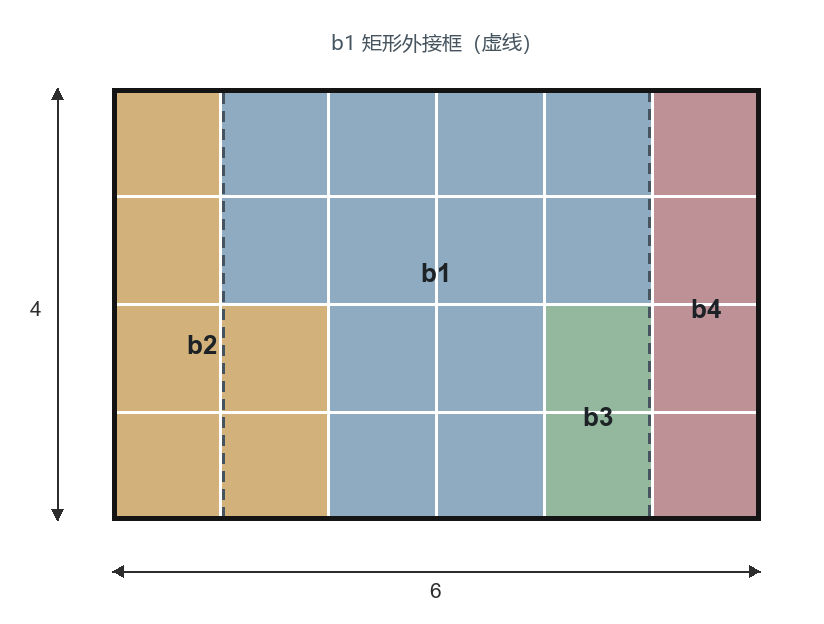
\includegraphics[width=0.76\textwidth]{../results/q4/figures/q4_optimal_layout.png}
  \caption{四个模块利用 b1 凹槽形成的 $6\times4$ 全局最优形状级布局}
  \label{fig:q4_optimal_layout}
\end{figure}

图中，b2 的右下短臂进入 b1 外接框左下方未被 T 型实体占据的凹槽，旋转 $90^\circ$ 的 b3 则进入其右下凹槽；最终真实占用区域均位于轮廓内且两两不交。由此可见，形状级碰撞判定能够利用非矩形模块的凹槽空间，而矩形外接框模型会错误排除这一零死区布局。

因此，本问通过真实形状集合建模利用凹槽，并以“面积下界 $24$ + 面积为 $24$ 的具体构造”严格证明了 $6\times4$ 布局的全局最优性。
